\section{Attention-based pooling with \ournet}
\label{sec:architecture}

\begin{figure*}[ht]
    \centering
     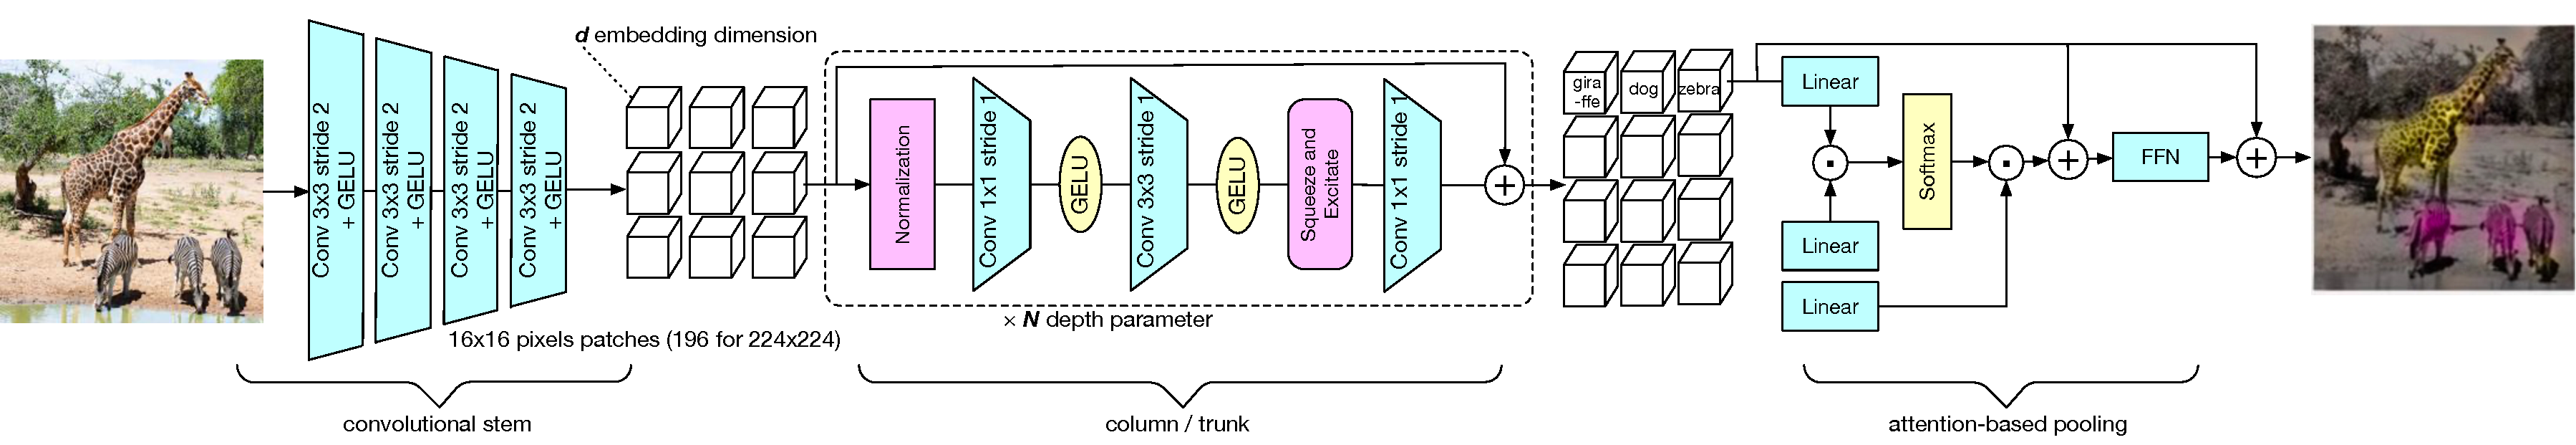
\includegraphics[width=1.0\linewidth,clip,trim=0 0 0 0pt]{figs/patchconv.pdf}
    \caption{Detail of the full model, with the convolutional stem on the left, the convolutional main block in the middle, and here toppled with multi-class attention-based pooling on the right.
    \label{fig:full_model}}
\end{figure*}

The learned aggregation layer is best associated with a high-resolution feature map. Therefore, while it can be combined with any convolutional architecture like a regular ResNet-50, our suggestion is to combine it with an architecture that maintains the resolution all across the layers. Some works exist, however they offer an underwhelming trade-offs~\cite{tolstikhin2021MLPMixer,Touvron2021ResMLPFN}. To remedy to that problem, we introduce \ournet. This design, which illustrated in Figure~\ref{fig:full_model}, 
is intended to concentrate most of the compute and parameters in the columnar trunk. 
The architecture family is parametrized by the embedding dimension $d$, and the number of repeated blocks in the trunk $N$. 
Below, we describe the architecture and its training in more details.  

\subsection{Architecture design}



\paragraph{The convolutional stem} is a light-weight pre-processing of the image pixels whose role is to segment and map an image into a set of vectors. 
In ViT, this exactly corresponds to the patch extraction step~\cite{dosovitskiy2020image}.
Therefore, we refer to the vectors resulting from this pre-processing as \emph{patches}. 
Recent papers~\cite{graham2021levit,el2021xcit} have shown that it is best to adopt a convolutional pre-processing, in particular for stability reasons~\cite{xiao2021early}. 
In our case, we borrow the convolutional stem from LeVit~\cite{graham2021levit}: a small ConvNet that is applied to the image of size $W\times H \times 3$ and produces a vector map of $W/16 \times H/16 \times d$. 
It can be viewed as a set of $k$ non-overlapping $d$-dimensional patches. 
%
In our experimental results, except if mentioned otherwise, we use a convolutional stem consisting of four $3\times3$ convolutions with a stride of $2\times2$, followed by a GELU non-linearity~\cite{Hendrycks2016GaussianEL}.
We illustrate the convolutional stem in Figure~\ref{fig:full_model}.

\paragraph{The column,} or trunk, is the part of the model which accounts for most of the layers, parameters, and compute. 
It consists of $N$ stacked residual convolutional blocks as depicted in Figure~\ref{fig:full_model}. 
The block starts with a normalization, followed by a $1\times1$ convolution, then a $3 \times 3$ convolution for spatial processing, a squeeze-and-excitation layer \cite{Hu2017SENet} for mixing channel-wise features, and finally a $1\times1$ convolution right before the residual connection. 
Note that we can interpret the $1\times1$ convolutions as linear layers.
A GELU non-linearity follows the first two convolutions. 
The output of this block has the same shape as its input: the same number of tokens of the same dimension $d$.

Using BatchNorm~\cite{ioffe15batchnorm} often yields better results than LayerNorm~\cite{ba2016layer}, provided the batches are large enough. 
As shown in Section~\ref{sec:experiments}, we also observe this for our model family. 
However, BatchNorm is less practical when training large models or when using large image resolutions because of its dependency on batch size.
In that setup, using BatchNorm requires an additional synchronization step across multiple machines. 
This synchronization increases the amount of node-to-node communication required per step, and in turn, training time. 
In other situations, like for detection and segmentation, the images are large, limiting the batch size and possibly impacting performance. 
Because of all those reasons, unless stated otherwise, we adopt LayerNorm.

\paragraph{Attention-based pooling.} 
At the output of the trunk, the pre-processed vectors are aggregated using a cross-attention layer inspired by transformers.
We illustrate this aggregation mechanism in Figure~\ref{fig:full_model}. 
A \emph{query} class token attends to the projected patches and aggregates them as a weighted summation. 
The weights depend on the similarity of projected patches with a trainable vector (CLS) akin to a class token. 
The resulting $d$-dimensional vector is subsequently added to the CLS vector and processed by a feed-forward network (FFN). 
As opposed to the class-attention decoder by Touvron \etal\cite{touvron2021going} we use a single block and a single head. 
This drastic simplification has the benefit of avoiding the dilution of attention across multiple channels. 
Consequently, the communication between the class token and the pre-processed patches occurs in a single softmax, directly reflecting how the pooling operator weights each patch. 

We can easily specialize the attention maps per class by replacing the CLS vector with a  $k \times d$ matrix, where each of the $k$ columns is associated with one of the classes. 
This specialization allows us to visualize an attention map for each class, as shown in Figure~\ref{fig:visu_attention}. 
The impact of the additional parameters and resulting FLOPS is minimal for larger models in the family. 
However, this design increases peak memory usage and makes the optimization of the network more complicated.
We typically do that in a fine-tuning stage with a lower learning rate and smaller batch size to circumvent these issues. 
By default, we use the more convenient single class token. 


\subsection{Discussion: analysis \& properties}
\label{sec:analysis}

\begin{figure*}[h!]
\vspace{-1.5ex}
\begin{minipage}{0.32\linewidth}
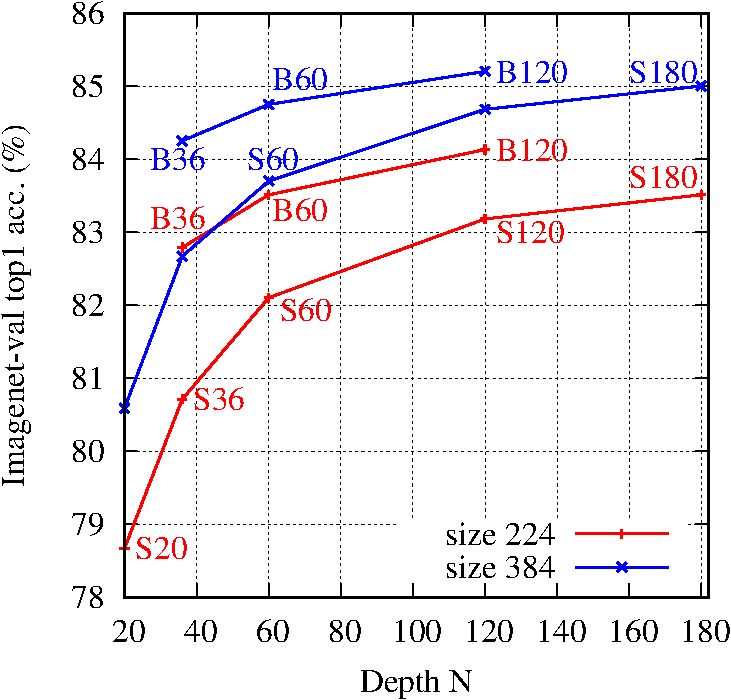
\includegraphics[width=\linewidth]{figs/acc_vs_depth_width}
\caption{Analysis of the accuracy as a function of width (S: $d$\,$=$\,$384$, B: $d$\,=\,$768$) and depth $N$. Depending on the performance criterion (importance of latency, resolution, FLOPs), one could prefer either deeper models or wider models. See Bello \etal ~\cite{Bello2021RevisitingRI} for a study on the relationship between model size, resolution and compute. 
\label{fig:acc_vs_depth_width}} 
\end{minipage}
\hfill
\begin{minipage}{0.32\linewidth}
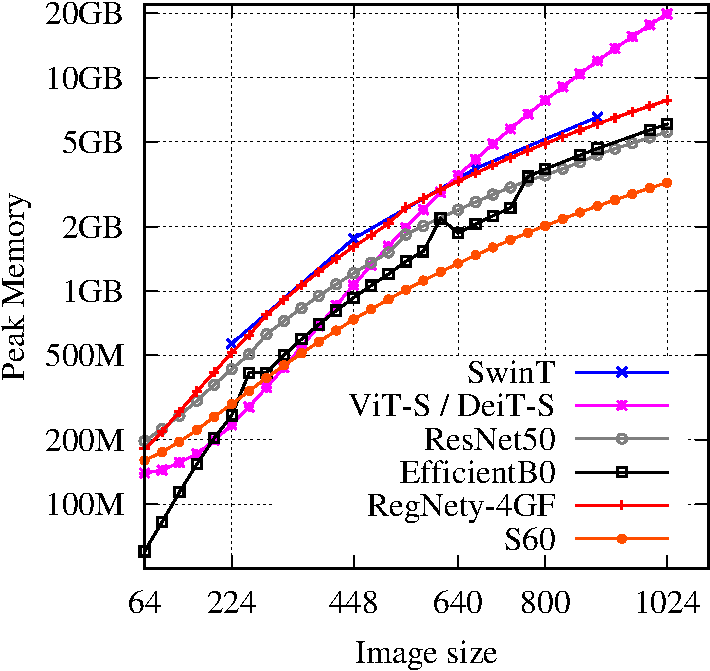
\includegraphics[width=1.02\linewidth]{figs/memory_vs_resolution}
\caption{Peak memory for varying resolution and different models. Some models like Swin require a full training at the target resolution. Our model scales linearly as a function of the image surface, like other ConvNets. This is in contrast to most attention-based models, which abide by a quadratic complexity for images large enough. 
%
\label{fig:mem_vs_resolution_S60}} 
\end{minipage}
\hfill 
\begin{minipage}{0.32\linewidth}
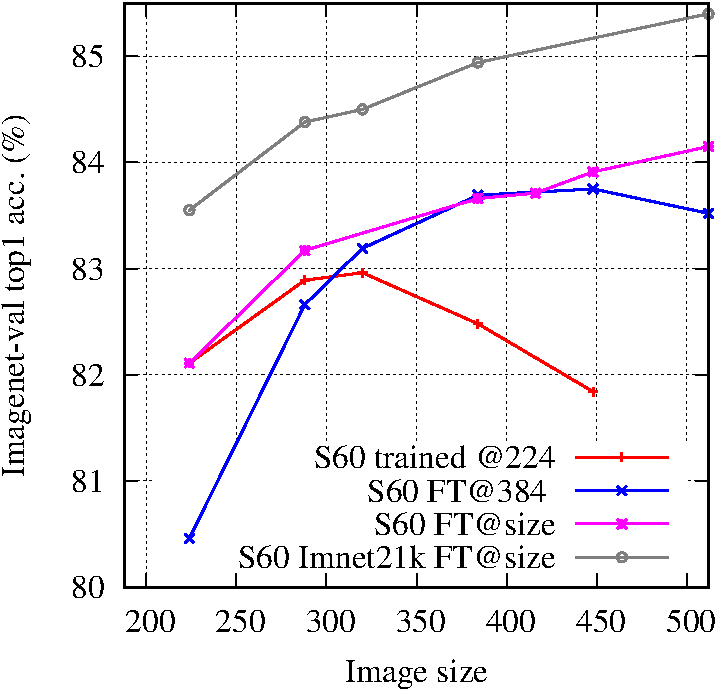
\includegraphics[width=\linewidth]{figs/acc_vs_resolution_S60}
\caption{Accuracy at different resolutions for the S60 model. We analyze models \textcolor{red}{trained at size 224} or \textcolor{blue}{fine-tuned (FT) @384}, and compare them to \textcolor{magenta}{models fine-tuned at the target inference size} to show the tolerance to test-time resolution changes. 
The \textcolor{black!70}{best model are pre-trained on ImageNet21k} at 224 or 320 and fine-tuned at test-time resolution. 
\label{fig:acc_vs_resolution_S60}} 
\end{minipage}
\vspace{-1.5ex}
\end{figure*}


Below we discuss several properties of our convolutional trunk augmented with the proposed attention-based aggregation stage. 


\begin{enumerate}
\item \emph{Simple parametrization.} Our main models are fully defined by width and depth. %
See Figure~\ref{fig:acc_vs_depth_width} for results obtained with these models at two different resolutions (224 and 384). 
Following the same convention as in previous work on vision transformers and vision MLPs~\cite{dosovitskiy2020image,Touvron2020TrainingDI,Touvron2021ResMLPFN}, we refer by S the models with an vector size of $d$\,$=$\,$384$ per patch, by B when $d$\,$=$\,$768$, and by $L$ for $d$\,$=$\,$1024$. 
We use the S60 model for most of our ablations and comparisons since it has a similar number of parameters and FLOPs as a ResNet-50. 

\item \emph{Visualization.} 
Our model allows to easily visualize the network activity. 
Saliency maps are directly extracted from our network without any post-processing. 

\item \emph{Constant resolution across the trunk.} 
The patch-based processing leads to a single processing resolution in the trunk. 
Therefore the activation size is constant across the whole network. 
The memory usage is (almost) constant at inference time, up to the pre- and post-processing stage, which are comparatively less demanding. 
Compared to traditional ConvNets, the network has a coarser processing in the early stages, but a finer resolution towards the output of the trunk. 

\item \emph{Linear scaling with image size.} 
This is a key difference with Vision Transformers. 
Pyramidal transformers such as LeVit, SwinTransformer or MViT partly solve the problem by breaking the quadratic component by rapidly down-scaling the image. 
However, they don't avoid the memory peaks happening with very large images. 
%
As a consequence of that constant memory usage and linear scaling, our model smoothly scales to larger resolutions, as shown in Figure~\ref{fig:mem_vs_resolution_S60} where we report the Peak Memory usage as a function of the image size.

\item \emph{Easy change of resolution}. 
We do not require any positional encoding, as the relative patch positions are handled by the convolutions. 
%
In that respect our approach is more flexible than most approaches that needs to be fine-tuned or trained from scratch for each possible target resolution. 
In Figure~\ref{fig:acc_vs_resolution_S60} we show that the properties of our models are quite stable under relatively significant resolution changes. 

% 
\item \emph{No max-pooling.} 
There is no max-pooling or other non-reversible operator in our architecture. 
Formally the function implemented by the trunk is bijective until the aggregation stage. 
We do not exploit this property in this paper, but it may be useful in contexts like image generation~\cite{Donahue2019LargeSA,Kingma2018GlowGF}. 

%
\end{enumerate}





\subsection{Training recipes} 
\label{sec:training_recipes}

% 
Like many other works (see Liu et al. \cite{liu2021survey}, Table I), our training algorithm inherits from the DeiT~\cite{touvron2021going} procedure for training transformers. 
We adopt the Lamb optimizer~\cite{you20lamb} (a variant of AdamW~\cite{Loshchilov2017AdamW}) with a half-cosine learning schedule and label smoothing \cite{Szegedy2016RethinkingTI}.
For data augmentation, we include the RandAugment~\cite{Cubuk2019RandAugmentPA} variant by Wightman \etal~\cite{wightman2021resnet}, Mixup~\cite{Zhang2017Mixup} ($\alpha=0.8$) and CutMix~\cite{Yun2019CutMix} ($\alpha=1.0$). 
Notably, we include Stochastic Depth~\cite{Huang2016DeepNW} that is very effective for deep transformers~\cite{touvron2021going}, and for which we observe the same effect with our deep \ournet.  
We adopt a uniform drop rate for all layers, and we cross-validate this parameter on ImageNet1k for each model (scores in  Table~\ref{tab:layernorm_vs_batchnorm}). 
We also adopt LayerScale~\cite{touvron2021going}. 
For the deepest models, the drop-rate hyper-parameter (often called ``drop-path'') can be set as high as 0.5, meaning that we can potentially drop half of the trunk. 
A desirable byproduct of this augmentation is that it accelerates the training. 
Note that we do not use gradient clipping, Polyak averaging, or erasing to keep our procedure simple enough. 

We now detail some context-dependent adjustments, based on datasets (ImageNet1k or ImageNet21k), and training (from scratch or fine-tuned). Note that, apart our sensivity study, we use the same Seed 0 for all our experiments~\cite{wightman2021resnet} to prevent picking a ``lucky seed''~\cite{picard21luckyseed} that would not be representative of the model performance. 


\paragraph{Training on ImageNet1k.} We train during 400 epochs with a batch size of 2048 and a learning rate fixed at $3.10^{-3}$ for \emph{all models}.  Based on early experiments, we fixed the weight decay to 0.01 for S models and 0.05 for wider models, but practically we observed that the stochastic depth parameter had a preponderant  influence and the most important to adjust, similar to prior observations with ViT \etal~\cite{touvron2021going}. 
%
We use repeated augmentation~\cite{berman2019multigrain} only when training with this dataset.  %




\paragraph{Fine-tuning at higher resolutions.} We fine-tune our models at higher resolutions in order to correct the train-test resolution discrepancy~\cite{Touvron2019FixRes}, and to analyze the behavior of our models at higher resolutions. This can save a significant amount of resources because models operating at larger resolutions are very demanding to train. 
For fine-tuning, we use a smaller batch size of 1024 in order to compensate for the larger memory requirements. We fix the learning rate to $10^{-5}$, the weight decay to 0.01, and fine-tune during 10 epochs for all our models. 

\paragraph{Training on ImageNet21k.} We train during 90 epochs as in prior works~\cite{dosovitskiy2020image,liu2021swin}. We trained with a batch size of 2048 with a learning rate of $3.10^{-3}$ and weight decay of 0.01, or when possible with a batch size of 4096 to accelerate the training. In that case we adjust the learning rate to $4.10^{-3}$. 
%

\paragraph{Fine-tuning from ImageNet21k to ImageNet1k} is a more involved modification of the network than just fine-tuning across resolutions because one needs to re-learn the classifiers. In that case, we adopt a longer fine-tuning schedule of 100 epochs %
along with a batch size of 1024 and an initial learning rate of $5.10^{-4}$ with a half-cosine schedule. 

